% !TeX root = main.tex

% abtex2-modelo-artigo.tex, v-1.9.2 laurocesar
% Copyright 2012-2014 by abnTeX2 group at http://abntex2.googlecode.com/
%

% ------------------------------------------------------------------------
% ------------------------------------------------------------------------
% abnTeX2: Modelo de Artigo Acadêmico em conformidade com
% ABNT NBR 6022:2003: Informação e documentação - Artigo em publicação
% periódica científica impressa - Apresentação
% ------------------------------------------------------------------------
% ------------------------------------------------------------------------

\documentclass[
	% -- opções da classe memoir --
	article,			% indica que é um artigo acadêmico
	11pt,				% tamanho da fonte
	twoside,			% para impressão apenas no verso. Oposto a twoside
	a4paper,			% tamanho do papel.
	% -- opções da classe abntex2 --
	%chapter=TITLE,		% títulos de capítulos convertidos em letras maiúsculas
	%section=TITLE,		% títulos de seções convertidos em letras maiúsculas
	%subsection=TITLE,	% títulos de subseções convertidos em letras maiúsculas
	%subsubsection=TITLE % títulos de subsubseções convertidos em letras maiúsculas
	% -- opções do pacote babel --
	english,			% idioma adicional para hifenização
	brazil,				% o último idioma é o principal do documento
	sumario=tradicional
	]{abntex2}


% ---
% PACOTES
% ---

% ---
% Pacotes fundamentais
% ---
\usepackage{lmodern}			% Usa a fonte Latin Modern
\usepackage[T1]{fontenc}		% Selecao de codigos de fonte.
\usepackage[utf8]{inputenc}		% Codificacao do documento (conversão automática dos acentos)
\usepackage{indentfirst}		% Indenta o primeiro parágrafo de cada seção.
\usepackage{nomencl} 			% Lista de simbolos
\usepackage{color}				% Controle das cores
\usepackage{graphicx}			% Inclusão de gráficos
\usepackage{microtype} 			% para melhorias de justificação
% ---
\usepackage{hyperref}
\usepackage{amsmath}
\usepackage[showframe]{geometry}
\usepackage{bm}


% ---
% Pacotes adicionais, usados apenas no âmbito do Modelo Canônico do abnteX2
% ---
\usepackage{lipsum}				% para geração de dummy text
% ---

% ---
% Pacotes de citações
% ---
\usepackage[brazilian,hyperpageref]{backref}	 % Paginas com as citações na bibl
\usepackage[alf]{abntex2cite}	% Citações padrão ABNT
% ---
% ---
% Configurações do pacote backref
% Usado sem a opção hyperpageref de backref
\renewcommand{\backrefpagesname}{Citado na(s) página(s):~}
% Texto padrão antes do número das páginas
\renewcommand{\backref}{}
% Define os textos da citação
\renewcommand*{\backrefalt}[4]{
	\ifcase #1 %
		Nenhuma citação no texto.%
	\o
		Citado na página #2.%
	\else
		Citado #1 vezes nas páginas #2.%
	\fi}%
% ---

% ---
% Informações de dados para CAPA e FOLHA DE ROSTO
% ---
\titulo{Matéria escura e energia escura}
\autor{Tiago H. B. Alves\texorpdfstring{\thanks{tiagohbalves@hotmail.com}}{}}
\local{Brasil}
\data{2024}
\def\assunto{Assunto}
% ---

% ---
% Configurações de aparência do PDF final

% alterando o aspecto da cor azul
\definecolor{blue}{RGB}{41,5,195}

% informações do PDF
\makeatletter
\hypersetup{
     	%pagebackref=true,
		pdftitle={\@title},
		pdfauthor={\@author},
    	pdfsubject={\assunto},
	    pdfcreator={\@author},
		pdfkeywords={abnt}{latex}{abntex}{abntex2}{atigo científico},
		colorlinks=true,       		% false: boxed links; true: colored links
    	linkcolor=blue,          	% color of internal links
    	citecolor=blue,        		% color of links to bibliography
    	filecolor=magenta,      		% color of file links
		urlcolor=blue,
		bookmarksdepth=4
}
\makeatother
% ---


\ifthenelse{\equal{\ABNTEXisarticle}{true}}{%
\renewcommand{\maketitlehookb}{}
}{}
% ---
% compila o indice
% ---
\makeindex
% ---

% ---
% Altera as margens padrões
% ---
\setlrmarginsandblock{3cm}{3cm}{*}
\setulmarginsandblock{3cm}{3cm}{*}
\checkandfixthelayout
% ---

% ---
% Espaçamentos entre linhas e parágrafos
% ---

% O tamanho do parágrafo é dado por:
\setlength{\parindent}{1.3cm}

% Controle do espaçamento entre um parágrafo e outro:
\setlength{\parskip}{0.2cm}  % tente também \onelineskip

% Espaçamento simples
\SingleSpacing

% ----
% Início do documento
% ----
\begin{document}

% Retira espaço extra obsoleto entre as frases.
\frenchspacing

% ----------------------------------------------------------
% ELEMENTOS PRÉ-TEXTUAIS
% ----------------------------------------------------------

%---
%
% Se desejar escrever o artigo em duas colunas, descomente a linha abaixo
% e a linha com o texto ``FIM DE ARTIGO EM DUAS COLUNAS''.
% \twocolumn[    		% INICIO DE ARTIGO EM DUAS COLUNAS
%
%---
% página de titulo
\maketitle

% resumo em português
\begin{resumoumacoluna}
 Dois dos maiores problemas atuais da cosmo

 \vspace{\onelineskip}

 \noindent
 \textbf{Palavras-chaves}: Matéria escura, energia escura, gravitação.
\end{resumoumacoluna}

% ]  				% FIM DE ARTIGO EM DUAS COLUNAS
% ---

% ----------------------------------------------------------
% ELEMENTOS TEXTUAIS
% ----------------------------------------------------------
\textual

% ----------------------------------------------------------
% Introdução
% ----------------------------------------------------------
\section*{Introdução}


O universo observado tal como conhecemos é constituído em quase toda sua totalidade por 3 ingredientes principais, ele é composto por\footnote{Os valores podem variar conforme a fonte, mas sempre se mantém próximo a essa proporção} \footnote{Também existe a componente de radiação, abundante e importante nos períodos iniciais do nosso universo, porém irrisória para a época atual}:

\begin{itemize}
	\item $\bm{5\%}$ de matéria bariônica;
	\item $\bm{27.5\%}$ de matéria escura;
	\item $\bm{67.5\%}$ de energia escura.
\end{itemize}

Com essas 3 componentes principais conseguimos descrever todos os fenômenos que observamos no universo, independente de escala. E todas as interações entre as componentes constituinte do nosso universo podem ser descritas a partir de 4 interações fundamentais, que são as interações forte, eletromagnética, fraca e gravitacional. Com essas interações tentamos conseguir descrever todos os fenômenos observados no universo, independentemente da escala utilizada.

\subsection*{Interação nuclear forte}

A interação forte como o próprio nome diz é a interação física com maior nível de intensidade que conhecemos, ela é principalmente responsável por manter os prótons estáveis, além de mantê-los junto com os nêutrons unidos no núcleo atômico. A sua compreensão é essencial para entendermos os processos de fusão e fissão nuclear, processos estes importantes para entendermos alguns dos efeitos que ocorrem dentro das estrelas e também em reatores nucleares.

A interação nuclear forte opera através das trocas de partículas chamadas glúons que carrega a interação entre os quarks. Uma das suas principais características é o seu curto alcance sendo da ordem do núcleo atômico $10^{-15}m$, sendo imperceptível em demais escalas do nosso universo.

\subsection*{Interação eletromagnética}
Em escala de magnitude das interações a eletromagnética fica logo após a interação nuclear forte. Ela é cerca $\frac{1}{137}$\footnote{Esse valor também é conhecido como constante de estrutura fina.\url{https://physics.nist.gov/cuu/Constants/alpha.html}} mais fraca que a nuclear forte.

A interação eletromagnética descreve a relação entre partículas carregadas eletricamente, como prótons, elétrons e outras partículas subatômicas que possuem carga elétrica. Essa interação é mediada pelo fóton. Diferente da interação forte seu alcance é considerado infinito.

Essa interação desempenha um papel fundamental em diversos fenômenos, desde a formação de átomos e moléculas até a transmissão de sinais elétricos e magnéticos. A interação eletromagnética é essencial para o funcionamento de muitas tecnologias modernas, incluindo eletricidade, eletrônica, comunicação sem fio e muitas outras.

\subsection*{Interação nuclear fraca}

A interação nuclear fraca é principalmente responsável por certos tipos de decaimento radioativo e pela interação entre partículas subatômicas, como nêutrons e prótons, dentro do núcleo atômico. Sua magnitude em comparação com a interação nuclear forte é da ordem de $10^{-13}$, assim como ela possui é de curto alcance, cerca de $10^{-18}m$

A interação fraca é mediada por partículas chamadas bósons $W^+$, $W^-$ e $Z^0$, eles são responsáveis por transmitir a força fraca entre as partículas.

Essa interação desempenha um papel crucial em fenômenos como o decaimento beta, na qual um nêutron se converte em um próton, um elétron e um antineutrino do elétron\footnote{Também é possível decair em um antipróton, um pósitron(anti elétron) e um neutrino do elétron.}, além de outras formas de decaimento nuclear. Além disso, a interação fraca é essencial para entender processos astrofísicos importantes, como a fusão nuclear que ocorre no interior das estrelas.

\subsection*{Interação gravitacional}

A interação gravitacional é a interação predominante nas grandes escalas do nosso universo, ela é principalmente responsável pela atração de todos os objetos que possuem massa, tendo um caráter exclusivamente atrativo, diferente da força	eletromagnética. De todas as interações ela é a que possui a menor magnitude, cerca de $10^{-38}$ em comparação com a nuclear forte, porém assim como a interação eletromagnética ela possui um alcance infinito.

A gravidade é fundamental para a formação e manutenção de sistemas astronômicos, como o nosso sistema solar, e influencia todos os aspectos do movimento dos corpos celestes.

Embora a gravidade seja a mais fraca das interações, ela é a principal interação que tenta descrever $95\%$ da composição do nosso universo e também é a interação que domina em grandes. Além disso das quatro interações fundamentais ela é mais desconhecida entre as outras.


\section{O que é a gravidade?}
A gravidade como visto é a interação principal que domina no cosmos. Porém ainda não sabemos sua origem nem seus mecanismos de interação entre os corpos com massa. A gravidade já teve diversas interpretações desde os primórdios com uma teoria aristotélica até os tempos modernos com a teoria de einstein.

\subsection{Teoria aristotélica da gravitação}

Aristóteles, foi um filósofo grego que desenvolveu diversas ideias sobre a natureza do mundo, incluindo algumas concepções sobre o movimento dos corpos e a gravidade. De acordo com a visão aristotélica, os corpos celestes, como planetas e estrelas, eram feitos de um elemento chamado "éter", que era diferente dos quatro elementos (terra, água, ar e fogo) que compunham os objetos terrestres. Ele acreditava que os corpos celestes eram perfeitamente esféricos e que se moviam em órbitas circulares e uniformes ao redor da Terra, que ele considerava o centro do universo, criando uma ideia de universo geocêntrico.

Para Aristóteles também o movimento dos corpos seria sempre em direção ao seu lugar natural, lugar este que seria de repouso. Então para Aristóteles uma pedra caía porque o lugar natural delas seria o chão, os astro estariam no céu pois lá seria o seu lugar natural.

Porém a teoria aristotélica era incapaz de explicar alguns fenômenos observado, como por exemplo o movimento dos demais planetas do sistema solar. Sendo necessário uma nova teoria para explicar esses fenômenos.

\subsection{Teoria newtoniana da gravitação}

A teoria gravitacional que seguiu após a teoria aristotélica foi a teoria newtoniana da gravitação. Essa teoria surgiu a partir da evolução do pensamento, com as ideias de inércia propostas por Galileu Galilei e posteriormente com a formulação gravitacional de Newton.

Para Newton a gravidade seria uma forca que atua sobre todos os corpos com massa essa forca serra proporcional a massa dos objetos e inversamente proporcional ao quadrado da distancia, dado pela equação
\begin{equation}
	F = \frac{Gm_1m_2}{r^2} .
\end{equation}
Com a formulação newtoniana da gravidade diversos eventos, que antes não se conseguia justificar pelas teorias aristotélica, foram explicados pela teoria de Newton. Descobrimos que os planetas possuem órbitas elípticas, em torno do sol, conseguimos descobrir o oitavo planeta do sistema solar, Netuno, e  que todos os corpos caem com mesma aceleração em direção a terra, diferente do pensamento anterior em que achava-se que quanto maior a massa maior seria a aceleração em direção a terra.

Porém mesmo sendo uma teoria que foi rapidamente aceita, a gravitação newtoniana havia alguns problemas, além dela por sí só não descrever a órbita completa de Mercúrio, ela também causava uma estranheza por ser uma força de ação instantânea, por isso se fazia necessário uma teoria gravitacional capaz de explicar tais fenômenos. A próxima teoria gravitacional que surge é a teoria gravitacional de Einstein chamada da teoria da relatividade geral.
\subsection{Teoria da relatividade geral}

A teoria da relatividade geral, traz um novo pensamento para a  física, nela a gravidade não é apenas uma forca que interage entre todos os corpos mas sim uma deformação do espaço, também na teoria da relatividade é proposto que o espaço ao invés de ter as 3 dimensões previamente conhecidas, era na real composto por 4 dimensões, que seriam 3 dimensiones espaciais e uma temporal.

Com isso na relatividade geral a gravidade passa de ter um caráter exclusivamente físico e se torna uma teoria geométrica, tornando-se também uma propriedade do espaço tempo, para isso Einstein surge com sua famosa equação\footnote{De fato essa equação está sumarizada e contém na verdade em seu significado um total de 16 equações que correspondem  ao conjunto total.}
\begin{equation}
	R_{\mu \nu}+\frac{1}{2}g_{\mu \nu} R = T_{\mu \nu},
\end{equation}

ao qual podemos é dividida em dois lados, no lado esquerdo contém a parte de geometria, na qual define como o espaço se curva e no lado direito da equação em como a matéria curva o espaço.

Em consequência da característica geométrica da gravidade, consegui-se justificar a órbita de mercurio, que por estar mais perto do sol sentia o campo gravitacional de maneira diferente dos demais, alterando o seu perielio. E também descobriu novos efeitos causados pela gravidade, entre eles o lenteamento gravitacional.

O lentiamento gravitacional é um efeito causado pela deformação da luz ao passar por um campo gravitcional bem forte. A luz, como se sabe, possui uma trajetória em linha reta, porém, como a gravidade curva o espaço, ela também curva a trajetória do raio de luz, faznedo a função de uma lente. Esse efeito foi primeiramente observado em sobral em 1919, que foi o primeiro experimento que comprovou a teoria da relatividade geral e também é um fenômeno importante para entendermos o comportamento de graneds estruturas.

\begin{figure}\centering
	\caption{Diagrama de uma lente gravitacional, mostrando como a luz e uma galáxia distante, ou uma estrela, pode ser curvada devido a interação gravitacional.}
	\includegraphics[width=10cm]{lens.pdf}
	\centering
	{\par \footnotesize Fonte: NASA, ESA, Ann Feild (STScI), Frank Summers (STScI)
		}
\end{figure}

A teoria da relatividade geral é a teoria gravitacional mais recente que temos, ela consegue descrever uma grande gama de fenômenos cosmológicos no nosso universo. Porém ela falha em descrevê-lo como um todo. Existem dois fenômenos importantes que a relatividade geral as demais interáções físicas não descrevem, que são a energia escura e a matéria escura. Que são dois fênomenos que não conseguimos medir seus efeitos no nosso sisetma solar mas de suma importância para o universo como um todo. 

\section{Matéria escura}

A matéria escura é um dos principais problemas em aberto da física moderna e da cosmologia, a primeira indicação da sua presença
pode ser encontrada no estudo da dinâmica de nossa galáxia. Em 1922 Jacobus Kaptey calculo a densidade
de matéria perto do Sol e também estimou a densidade de todo o plano galático\cite{1922ApJ55302K}. Kaptey concluiu que a densidade
de matéria obtida em seus cálculos era o suficiente para explicar o movimento vertical das estrelas pŕoximas ao plano galáctico. Porém no mesmo ano, James Jeans
ao reanalizar o movimento dessas estrelas no plano vertical, concluiu que deveria haver duas "estrelas escuras" para cada estrela\cite{10.1093/mnras/82.3.122}, ou em outras palavras a massa total
da galáxia deveria ser o triplo do observado.

Em 1933 Fritz Zwicky ao medir as velocidades radiais no Superaglomerado de Coma, na constelação de Coma Berenice. Ao calcular a velocidade orbital das galáxias
Zwicky observou que a massa do cluster deveria ser maior, por um fator de 10, da massa observada do cluster\cite{1933AcHPh...6..110Z}. Ele concluiu que deveria existir uma
"matéria escura", invisível para nós, para que o aglomerado tivesse força gravitacional suficiente para manter as galáxias em órbita. No ano anterior o astrônomo
Jan Oort chegou á resultados semelhantes ao de Zwicky porém ele não postulou a existência de nenhuma matéra exótica como a matéria escura, porém outras evidências
da matéria escura refutam as ideias propostas por Oort.

O trabalho de Zwicky e a ideia proposta da matéria escura foi ignorados na sua época, ficando congelada por quase 40 anos. Foi apenas nos anos de 1970
que a ideia foi ressuscitada, quando astrônomos observaram o movimento de galáxias-satélite\footnote{pequenas
	galáxias próximas às grandes}, que só podiam ser explicadas pela presença de uma matéria adicional e invisível.
Mas seu status se concretizou de verdade a partir dos trabalhos de Vera Rubin, astrônoma do Instituto Carnegie, de Washington ,que trabalhou com o astrônomo Kent Ford. Depois da pós-graduação na Universidade de Georgetown,
Rubin decidiu medir o movimento angular de estrelas em galáxias \footnote{Inicialmenete  por Andrômeda}.
Ela e Kent Ford, descobriram que as
velocidades rotacionais das estrelas eram quase as mesmas a qualquer distância
do centro galáctico. Ou seja, as estrelas rotacionavam em velocidade constante,
mesmo que muito distantes da região que continha matéria luminosa. A única
explicação possível era uma matéria desconhecida que ajudava a conter
as estrelas mais distantes e a se movimentava bem mais rápido que o esperado. Sem
a existência dessa matéria, devido a alta velocidade, as estrelas seriam ejetadas das galáxias. O resultao obtido por eles foi de
que a matéria comum corresrespondia por apenas um sexto da massa
necessária para manter as estrelas em órbita.
Desde os anos 1970, as provas da matéria escura se tornaram ainda mais fortes e calculadas de maneira ainda melhor.
Entre os efeitos dinâmicos que nos possibilitam aprender sobre a matéria escura está a rotação das estrelas nas galáxias.
Contudo, essas medições se aplicavam apenas a galáxias do tipos espirais. Posteriormente foram verificados também os mesmos resultados para outro tipo de galáxias.
Como o avanço das medições elas começaram a ser realizdadas dez vezes mais longe dos centros das galáxias do que a extensão de matéria visível, elas
demonstraram não só que a matéria escura existe, mas que sua influêncua se estendia
muito além da parte visível de uma galáxia. Outras medições da temperatura e densidade
do gás, via raios X, confirmaram esse resultado.

\subsection{Próximas evidências}

A próxima pista da existência da matéria escura se originou na cosmologia, quando estuda-se um de seus pilasres, a expansão do universo.
A partir da expanão do universo é possível calcular a sua densidade crítica e comparar com a densidade média do universo. A partir dessa relação
é possíveel definir sua geometria, entre aberta\footnote{Curvatura negativa e relação<1.}, fechada\footnote{Curvatura positiva e relação>1} ou plano\footnote{Curvatura nula e relação igual a 1}.
A estimativa utilizando a matéria luminosa (utilizando esrtelas e o gás intraestelar ou extra estelar) é uma porcentagem pequena da densidade critica. Isto é consisetnte com os modelos da nuclosintese primordial.

Outra pilar da cosmologia é a distribuição de galáxias no universo. Nos primórdis da cosmologia pensava-se que a distribuição de galáxias seguiria um caráter randomico e que estariam distribuidas de maneira quase homogênea no espaço.
Porém com dados da distribuição descobriu que a distribuição das galáxias estão interligadas por filamentos, semelhantes a uma teia de aranha, e que o expaço entre os filamêntos são praticamente vazios. Podemos ver como se dá essa estrutura através da figura \ref{fig2}, onde conseguimos observar essa teia cósmica.

\begin{figure}\centering
	\caption{Teia cósmida da matéria escura, nela é possível ver os filamentos e a concentração de matérias nos vértices.}
	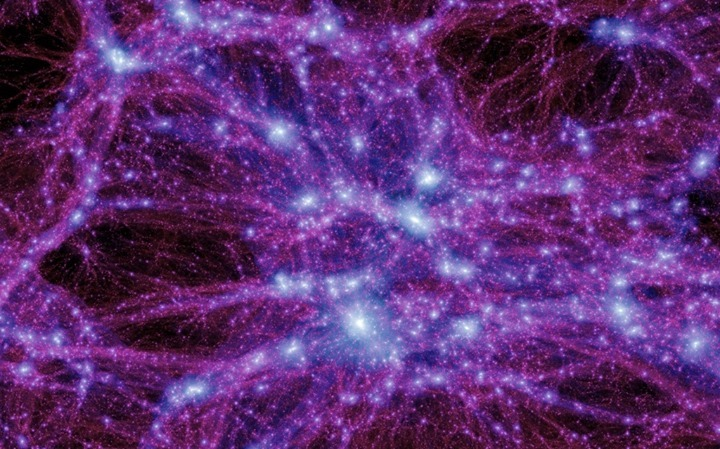
\includegraphics[width=10cm]{dark_net.png}\label{fig2}
	{\par FONTE: USDE, 2020}
\end{figure}

Tabém como vimos a gravidade curva a luz, causando o que chamamos de lentes gravitacionais, e as lentes gravitacionais também são um forte indicativo da existência da matéria escura, pois pela curvatura que é feita no raio de luz, quando este passa por uma galáxia conseguimos medir sua massa, e comparando com os valores obtidos a partir de sua intensidade luminosa também percebemos a sua divergencia.

Por fim, o indicativo mais significativo para nós sobre a existência da matéria escura, e também um indicativo da energia escura, é a própria idade do nosso universo. Se nosso universo fosse compsoto apenas por matéria bariônica ele seria velho demais com o que sabemos hoje em dia, ou a força gravitacional que fez a galáxias se formarem, seria menor impossibilitando a existência das galáxias em seu formato atual. 

\subsection{Alguns Candidatos}
Mas o que seria então a matéria escura? Até agora sabemos que a matéria escura tem se comporta gravitacionalmente no universo e que também não énenhuma interação com a luz, ou em outras palvras ela não possui interação com a força eletromagnética. Também sabemos que la está presente deste o início do nosso universo até os tempos atuais. 

Com isso temos alguns indicativos do que a matéria escura não pode ser. Sabendo como a matéria escura se comporta conseguimos fazer algumas predições a cerca de sua natureza e criar alguns modelos 
\section{Energia escura}

\section{Evidencias}
\section{Candidatos}



\section{Evidencias iniciais}
\subsection{Matéria escura local}



\chapter{Minha fala}
O Thiago é o mestre da oficina e vai falar para a gente sobre matéria e energia escura. Obrigado, Thiago. Vou aparecendo... E aí E aí Boa. Tarde, eu sou o Thiago, como eles falaram, e eu vou falar um pouco sobre o que é a matéria que reivindica esse programa. Como eu disse, eu sou aluno da Paz Paixão do Cosmo, sou aluno de mestrado, aluno da Universidade Federal. Então, a primeira questão que você vai se acostumar, eu vou dar uma primeira opera com a introdução. Depois eu vou falar um pouco sobre gravidade para inicializar apenas alguns termos que eu preciso que vocês entendam para poder explicar o que é energia escura e matéria escura. É mais voltatório ensinar o método, então a maioria das coisas vai ser mais contextual. Então vamos trabalhar a mão da matemática e mais, sei lá, gêneros que a gente sabe. Primeira coisa. O que é o composto do Universo conhecido? O que é o Universo que a gente tem? Inicialmente, a gente sabe que o Universo é 5\% de matéria chamada matéria planilha, que são estrelas, planetas, gases. Então todo o tipo de matéria que ela vai, reage com a luz. E que a gente sabe, tem noção do nosso dia a dia. Então, isso vai ser apenas 5\%, os outros 25\% é de matéria escura, que eu vou explicar depois essa denunciação e como foi feito. E por fim, que é o mais recente, que é 70\% de energia escura. Então, com tudo isso aqui, com toda essa composição, a gente tem que produzir Sabemos toda a nossa composição do nosso universo e com as raízes físicas a gente consegue ter uma noção de descrição delas. É claro que as raízes físicas a gente vai ter mais a matéria baiônica e hoje em dia a gente tenta definir o que é a matéria de registro e como essa matéria deve ser adequada. Mas antes, primeiro que é a gravidade, certo? A gravidade Ela é compondo as quatro forças ou interações fundamentais. As outras três, a nuclear forte, a eletromagnética, a nuclear fraca e gravitacional. Aqui a gente consegue ver uma noção da comparação entre cada força. Então, por exemplo, a força eletromagnética, ela é uma certeza da força nuclear. Enquanto a gravitacional é 10, em relação ao gráfico altitude, ela tem uma ordem de magnitude muito menor do que as outras. Enquanto também tem um alcance, pelo. Menos. A gente está vendo, a eletromagnética gravitacional, ela tem um alcance, podemos dizer, enfim, um alcance todo o universo. Enquanto as outras possuem um grau de alcançoura diferente daquelas, tem um alcance muito pequeno. que é a nucléia forte, ela não tem alcoolisol ou tal ali no átomo e a nucléia fraca, ela pode ser do núcleo para o venoso e a nucléia forte, ela vai aumentar tanto a ligação do núcleo com o núcleo dos prótons e dos neutrons para fazer a disposição dele que ela é como um fosso de quartzo um próton de dois átomos e um náutil um próton de dois átomos e um núcleo tanto para manter essa ligação exigem a força do gráfico fotográfico e também para uma construção do núcleo, porque como o próprio tem carga positiva no núcleo, deveria ser representada a força da eletromagnética. Mas como ele exige a força do gráfico fotográfico, se mantém. A eletromagnética, tudo que tem carga elétrica, então, com o celular, tudo em nossa dianteira que a gente está relacionado com as forças magnéticas, com a energia elétrica, e também quando a gente vem... Quando a gente vê cargas, celulares, dispositivos, etc. A nuclear fraca, ela vai afetar todos os partículos, mas a gente vai reparar ela mais quando vai ocorrer o decaimento do nêutron. Então como o nêutron pode ter decaimento próprio, que é quando o nêutron está isolado fora do muro, então vai ter um decaimento que vai ser resultado da interação nuclear fraca, e ela vai fazer essa decomposição. A gravitacional é uma interação que todo o corpo tem massa. Então qualquer objeto com massa vai sofrer pela interação gravitacional. Então, eu com a garrafa dentro, a gente está se atraindo gravitacionalmente um ao outro, só que por outros motivos a gente não coloca. Mas se colocassem dois objetos suspensos, sem nada do que é, exigiam um círculo atrás de um chão outro, nesse caso. Então, quando a gente fala da gravitação, a primeira pessoa que teve uma formulação de o que seria a gravidade foi Newton. Ele foi em século 17. Ele foi o primeiro que fez essa formulação. Antes havia uma ação filosófica de como seria a gravidade, só que Nada dava uma explicação do que seria, do que poderia ser Só tinha a concepção brega de que os corpos caem porque a origem natural deles é o chão Então todo corpo da substância que cai é o chão Só que o muro não explica, por exemplo, o muro como um pássaro ou um pão de fogo Nada disso, por exemplo Então, como o livro colocou a realidade Ele vai colocar que a gravidade vai ter uma força proporcional ao máximo entre esses dois lados. Então, fazendo essa interação. E ela é imensamente proporcional ao quadrado da distância. Então, eu só tenho dois pontos. Então, assim, também tem a noção de força e assim como eu atrago um ponto, outro ponto também me atraga. Então, qualquer relação que tenha com a massa vai ser feita. Essa era a interação com a profissão alta. Só que, olhando a turma e os funcionários, ela apresentava alguns problemas. Só que pra época ela não tinha aceitado o que ela descrevia. Ela descrevia como os corpos caem, ela conseguia descrever o movimento dos planetas, ela conseguia descrever a fase dos efeitos, ela não tinha aceitado, só que ela tinha alguns problemas. O primeiro problema que a gente tem é um problema de conceito, que é a gravidade número. Se você pega um equilíbrio, Ela é uma força instantânea. Então, se você tivesse, por exemplo, a gente na Terra. Que tem o Sol. Se o Sol desaparecesse naquele momento, a gente sempre. Morreria. Ou, se você desaparecesse na Terra, o seu sinal funcionaria instantaneamente. Só que, pensando no conceito de universo, essas coisas, as coisas serem instantâneas, elas. Causam um pequeno desconforto. Porque a mesma coisa com o Sol, por exemplo, o buraco lembra um século da galáxia, se ele desaparecesse a gente se sentiria, e ele está há milhões de anos hoje. E esse é um primeiro. O segundo também que é importante a gente falar, que é a apreciação da altura e curva, mais cedo eu acho que foi no século 14 ou 17. O que é essa condensação? A gente está muito mais rápido de ser livre do que se o processo fizesse por causa de um erro. Porque na órbita, no caso do sol com ponto de gravação máximo, ou a órbita de meio público, ela começa a se soltar com o tempo. Só que aqui, por exemplo, com a. Gravidade de luz, todos os problemas que a gente tinha com gravatação, a gente conseguia fazer correções adicionava massa de um clarinho no outro, conseguia fazer essas correções. Então, quando faz a primeira correção, eu acho, da alta de urânio, você acha que é duro. Você faz uma correção, você consegue determinar o número de uma lua ou outra. Só que, por acaso, os autores não conseguiam realizar esse tipo de correção. Então, era... as primeiras... Tem sido um. Pouco, ela explicava um pouco do nosso problema, só que um pouco ela foi não explicando alguns detalhes que foi necessário que houvesse uma outra acumulação de teoria profissional. Que é a próxima pessoa que vai fazer essa acumulação de teoria profissional, que vai ser o Flávio. Aí a primeira coisa que eu fiz foi formular a teoria do governo nacional. A primeira coisa que eu fiz foi formular a teoria do governo nacional. A primeira coisa que eu fiz foi formular a teoria do governo nacional. A primeira coisa que eu fiz foi formular a teoria do governo nacional. A primeira coisa que eu fiz foi formular a teoria do governo nacional. A primeira coisa que eu fiz foi formular a teoria do governo nacional. A primeira coisa que eu fiz foi formular a teoria do governo nacional. A primeira coisa que eu fiz foi formular a teoria do governo nacional. A primeira coisa que eu fiz foi formular a teoria do governo nacional. A primeira coisa que eu fiz foi formular a teoria do governo nacional. A primeira coisa que eu fiz foi formular a teoria do governo nacional. A primeira coisa que eu fiz foi formular a teoria do governo nacional. A primeira coisa que eu fiz foi formular a teoria do governo nacional. A primeira coisa que eu fiz foi formular a teoria do governo Nesse caso, ele tem um insight que é a teoria geométrica de espaço-tempo. Então, ele coloca que a gravidade é uma objetividade do espaço, ela vai estar intrinsecamente ligada ao espaço e, no caso, à massa do espaço. E também coloca o espaço com 4 dimensões, onde ele vai adicionar o tempo. Nesse caso, a gente vai ter as massas, elas vão distorcer o espaço em sua volta. E com isso, você vai ter o que é essa distorção, ela vai como, por exemplo, ela vai gerar voltas. Essa distorção vai ser sentida como que a gente vai ter noção de uma força gravitacional. Com isso, surge a... Com isso, como tem uma nova teoria da posição raro, acaba que abandona até a fórmula da antiga. Aí, com isso, surge a equação, que é chamada equação de Einstein. Onde cada elemento, cada... Aqui vai corresponder a uma parte da equação. Cada... Esses índices vão de 0 a 3. Então, no total, esse é um conjunto de 16 equações. que seriam descreveriam a interação com o celular, conforme conhecemos hoje em dia. Então, é o que temos no primeiro lado da equação. Ele é descrito como o lado comum, que mostra como o espaço se curva. E o segundo lado da equação é. O... E o segundo lado da equação é como essa massa vai reagindo no espaço. Só que como a Thais disse mais cedo, para Einstein, a função de célula da equação vai ter um caráter dinâmico. Só que a concepção filosófica, quando ele colocou a gravidade, não fazia sentido muito o universo dinâmico, ele precisava de um universo estático. Então, quando tinha 14 equações, vai ver que o universo dele deveria se contrair, ele deveria ter um caráter mais humano. Então, o que ele faz? Em 1917, ele vai adicionar um termo, que é o crescente cosmológico. O que esse. Termo vai fazer? Esse termo vai equilibrar a equação para que o universo dele não se contraia mais, que ele seja menos estável. Só que o que acontece? Esse termo ele só existe porque a gente adiciona, ele não tem nenhum significado na época exótica, não faz sentido, e adiciona o termo, que é o para corrigir. Só que como vai mais pra frente? Porém, quando o vídeo, ele diz, vamos analisar as faixas uniais, vamos procurar soluções para as faixas uniais, E esse chegou a uma função diferente, porque pra eles, fazer mais simples, eles não entenderam o que eles falaram nessa prática. E eles tentaram analisar essa dinamicidade. Então é que eles vão para o universo do Caetano, se expandindo. Chegando até onde de hoje o filme o início. Ele tinha hoje o Big Bang, pessoal. Mas na verdade seria nessa imagem onde a gente tem as eras atuais. E lá no filme o início a gente consegue compartilhar esse tempo e ter uma noção de que lá no início o universo começou com um pequeno ponto, enfim, muito intenso, extremamente intenso, e que é a parte que distribuiu essa expansão do universo. E aí, seria essa expansão. Em Pitfall, o vapor mexe com a expansão e corrobora com as ideias de. Friedmann até o fim. Esse aqui é outro. e como que ele mete essa expansão. Para fazer esse tipo de medição, basicamente você veria o que acontece com a frequência do órgão. Quando, por exemplo, a gente tem um oxigênio emitindo um som, ele está emitindo uma frequência diferente, mas característica dele. Quando ele está se aproximando da gente, a frequência fica mais alta. Por exemplo, o John, no caso de mim, E quando ele se afasta, a freqüência que ele não vê é o mesmo como o 21. Então, como se medir essa expansão? Aqui, por exemplo, é outro exemplo de efeito. Se a fonte estiver parada, ela só mede assim. E se ela estiver afasta, quando você aproxima a luz, a gente consegue medir, ver e perceber essa diferença. E como sabemos... Esse aqui é o T23, então não tem as medições. De grau 1, mas. Eu só vou colocar o T24. E como sabemos que essa é uma emissão? Quando a gente tem gases, assim, a maioria do universo, a maioria do universo é composto de hidrogênio. E quando a gente abre esse espaço de hidrogênio, existe a absorção dos técnicos, e ela vai, por muito tempo, montar essa linha para nós com essas linhas que são características. Cada arco tem uma linha de características, que é de níveis exigentes, que vai ter um relacionamento com o seu número, de up e down, que vai ter um relacionamento com o seu número. Então cada arco tem uma linha bonita. Outro modo de patch da solução, aí eu tenho um exemplo aqui. Se está expandindo, A tendência é que a frequência aumente. Se você estivesse se aproximando de nós, a frequência aumentaria e o tempo de onda diminuiria e o tempo do plasma. Só que acontece ao contrário. É quando está se aproximando. Agora é quando se aproxima, quando se distancia de nós. As galáxias, com o comprimento de um soludo, hidrogênio, ele vai ter um deslocamento do mesmo nível. Foi isso que foi medido. E com isso a gente sabia que o universo estava em expansão. Se ele tivesse estático, ele estaria... estaria fixo. E se ele estivesse se aproximando da gente, os galáxios, os deuses, ele estaria voltado próximo. No caso do Andrômeda, que estava se aproximando da gente, ela voltada para o Andrômeda. Mas a maioria das coisas é voltada para o TV. Mas aí fica a pergunta, como o universo se esconde? Porque, quando você pensa no universo de novo, ele tem um ponto de início, mas ele também tem uma evolução. Então, consegui pensar no que poderia se esconder de algumas maneiras. As duas primeiras formas seriam, ele se esconde inicialmente, depois ele volta para o trás, só que pode ser rápido ou acelerado. A segunda forma, ou seja, o segundo tipo de expansão seria uma expansão constante, o universo ele sai de um ponto e ele expande profundamente. E o terceiro e o terceiro tipo seria o universo expandindo aceleradamente, porque ele começa a expansão e com o tempo ele vai só se acelerando nessa expansão. Até na década de 90, se tinha noção, não tinha noção, porque acreditava-se que a maioria do universo, a expansão dele seria mais acelerada, porque ele também. Existe. A nossa visão filosófica de que nos outros dois últimos casos, as coisas estão se afastando da gente e elas causam um tempo de serossimilitude. As coisas estão ficando cada vez mais distantes. Então, no futuro, causam essas estranhas... Porém, na década de 90, o trabalho... Na década de 90, com os resultados de supernovas, se descobriu que o universo estava em situação exagerada. Ou seja, a cada momento as coisas se distanciam mais e a velocidade de distanciamento dela também se aumenta. E foi descoberto pelo Dr. Norman Weiss-Giesemann que os alunos supernovas que tinham criado pra fazer esse tipo de negócio. E essa metáfora que a gente ligar, ela é utilizada como vela padrão nesse negócio. Ela é chamada de vela padrão, porque ela tem muito característico, muito celular, que a gente consegue fazer eleições precisas de quanto tá esse deslocamento em relação ao negócio. Aqui, por exemplo, olha o intervalo. De. Um ponto de... é logo depois ela desaparece. Só que o que que acontece? O que que causaria nessa expansão? Aí que surgiu agora a energia escura. A energia escura, nessa construção mais atual, ela seria uma componente do universo. Ela seria uma componente que seria responsável dessa expansão acelerada. Então, antes disso, como tinha essa noção? Então, a energia escura dela seria alguma coisa além do que a gente conhece, do que a gente observa, que ela está causando essa expansão. Então, como que seria? A gente tem a noção do mundo. Os galáxios, cada vez, estão ficando cada vez mais distantes. Então, se a gente pensar na física, a gente tem a noção do mundo mesmo como um sistema fechado. Então, se a gente tivesse um sistema fechado, a energia do mundo aqui, ela deveria manter o equilíbrio, assim dizer. Então, essa expansão deveria ser acelerada. Então, quando a gente coloca a concepção da energia, é por ser o somar do PGM que causa essa aceleração. Então, como a gente sabe, a primeira. Vez que o PGM soou foi com. O supernova do tipo A. A supernova do tipo A, ela vai ocorrer em sistema binário, onde você vai ter uma estrela menor, mais ou menos do tamanho do Sol, Porque no fim da vida dela, ela se torna uma água branca. Só que no fim, quando ela se torna uma água branca, ela começa a atualizar a gigante vermelha. Ela começa a atrair matéria dessa gigante vermelha. Aí começa a fazer as coisas lá, de gravidade, de puxar. surgindo, aí só que chegou um momento, o sistema normal sai de cima do trigo, e essa supernova, ela vai explodir. A não-branca, ela vai explodir, e ela vai virar supernova. Não é IA, é IA. Então, ela vai explodir. O segundo jeito que a gente sabe é pela CMV, que é a reação cósmica de fundo, porque a gente consegue medir o desvio que tem desses fósforos, que é a primeira imagem que a gente tem visível do nosso universo. Então a gente consegue medir essa imagem E a gente consegue medir o fondo distante com uma brilhante distância. Também a gente percebeu que ele também está afastando. Então a acenda dela, a cada tempo ela vai sendo deslocada mais para o vermelho. Para o vermelho, até como outra rede funcionosa, mas deve ser que vai ser muito pequena. e com essa filosofia a gente conseguiu perceber também a expansão do Universo. O fio, que é o mais recente, que chamamos de associação acústica ao Pai. Bem para o princípio do sucesso do Universo, não existiam elementos químicos, não existiam átomos, mas existiam as partículas de átomos. Só que chegou um momento que o Universo estava crescendo suspendido. Porém você tinha duas coisas acontecendo, você tinha altas temperaturas das partículas em alta velocidade querendo se expandir e você tinha gravidade tentando contrair ela. Então com essa contração gravitacional, puxado de gravidade, só que como puxado? Isso está a ver com o efeito de uma onda, que a gente consegue medir. Que a gente tenha esse oposto mesmo dessas ondas, assim. Que a gente tenha essa medição como também ela serve como um modelo padrão. Onde a gente tem uma boa medição sobre qual é a taxa de situação. Que a gente quer. Então, o que poderia ser essa energia escura? Existe quatro trilhas de água. e tento explicar o que é que só devem ser. Existem, é claro que existem, muito mais teorias, mas elas podem ser justificadas nessas quatro principais. A primeira que seria bastante normal, eu acho que seria só um termo adicional da gravitação. Embora o mais grande sonoro graficar é estático, seria um termo que existe, então a universidade expandiria porque ele se expande. O segundo seria um campo escalar, que ele seria... que ele funcionaria inversamente, na verdade, se ele não existisse. Ele estaria somando essa aceleração e faria as coisas semanalmente. O terceiro são as teorias de gravitação modificadas, que é a mesma alternativa, que realmente vão explicar qual outro formato, qual outro jeito poderia justificar, que poderia ser um outro teorema de notação, ou poderia ser outra concepção de notação. E também tem a questão de ser uma quinta força do protocolo, no sentido de para dançar uma parte desconhecida, por. Exemplo. A regia escura poderia ser mais um título que a gente não conhece, ela pode ter reiterações que a gente não conhece, e ela poderia ser um ponto dessa parte, fazer dançando o resultado dela. Eu expliquei que o Universo não se expandiu. Só que se o Universo se expandiu, se não movia-se a luz, se expandiu um pouco, o que que fez surgir, por exemplo, galáxias? O que que fez a Matéria se aglutinar? O que poderia ser feito? Porque se ele fizer, as coisas vão se expandindo. Então, desde o começo não deveria formar. Não deveria formar. Porque ele surge na matéria escura. Então, a matéria escura tem uma história antes da gravação. Na matéria escura ela tem uma história antes da energia escura. Ela vai começar primeiramente em 2012, onde vai ter um jogo do SKF, como eu disse. Eles estavam fazendo... Meio que saindo... Eles estavam fazendo, tentando calcular a densidade do som e a densidade de bateria. Só que... Então, ambos, ambos querem primeiro ter conta de uma discrepância de matéria. O Dieser acha essa discrepância de matéria. O Dieser acha essa discrepância de matéria, que poderia ser, poderia pensar assim. Só que ele não faz nenhuma conjectura de matéria. Ele só pensa que pode ser algum tipo de matéria que poderia ser a matéria comum, só que poderia ser um planeta, ou estrelas novas, ou outras coisas. Então, o Kepler, eu acho, ele refaz as contas do Kepler, e ele acha que deveria, que a matéria comum poderia. Ser uma matéria comum. Só que, em 23, 18, Ele, analisando o cluster coma, que é o cluster, ele vai ser um conjunto de galáxias. Então, ela vai ter o mesmo comportamento tanto de um sistema solar, onde você vai montar algo no centro, quanto também de uma galáxia. Ele, analisando o cluster, ele chegou à conclusão que a órbita, a velocidade dos corpos, as extremidades, era muito mais rápido do que seria o que ele estava medindo. Porque a gente mede a massa a partir da densidade luminosa dela. E a gente pega isso e calcula, consegue ter a noção da dotação. Só que eu percebi logo que as coisas, principalmente nas experimentais da galáxia, do cróstero educado, elas só davam muito mais rápido do que deveriam ser. Então ele propôs que deveria haver essa matéria invisível, que seria a matéria escura. E só um pequeno discurso, é que a gente usa o termo matéria escura, mas mais correto, seria matéria transparente, alguma outra coisa. Porque quando a gente observa, ela não reage com a luz. Quando a gente tem a noção de matéria escura, a gente tem a noção de que ela seria escura. mas ele coloca que seria um material invisível, que não seria constituído de nada. Que a gente... Então, entre isso e. 73 e 70, vai ter diversos trabalhos que vão colaborar com a ideia do... Só que a dívida diversa que se escreve nessas notácias não existe, não existia nada, não tinha um consenso sobre o que poderia causar. Muita gente pensava que podia ser erro estatístico notado, podia ser erro que propagou tanto na medida quanto nas contas, podia ser várias coisas. Mas só em 1470, que foi com o trabalho da Bergeron, e os novos dados que ela fez uma análise maior, verificou essa discrepância entre as matérias. Então, quando a gente pegar a observação, a gente tem essa curva, que toda vez que eu vejo matérias escuras, eu tenho essa curva em todo o quadro. Então você tem que ver a matéria que a gente observa, e em preto em vez de em verde, a matéria deveria ser observada para justificar essa velocidade orbital. E por que disso? Outra coisa, se não tivesse esse tanto de matéria, Esse é o meu primeiro ponto, o que isso deveria ser e como é. Se eu não tivesse esse tanto de matéria, as estrelas, todos os copos na conta, eles seriam ejetados do fora da galáxia porque eles estão em alta velocidade. Então, se você está em alta velocidade, ele vai ser ejetado porque não tem força gravitacional suficiente para manter o sistema. A segunda observação que depois foi ter foi com leites gravitacionais. Lá no começo eu disse que a matéria curva o espaço. Então ela também vai curvar a luz. Ela deveria ter uma trajetória reta, só que com essa curvatura do espaço que vai ter no corpo, ela também vai ter essa curvatura e também vai pegar a luz. Então, por exemplo, o que acontece? Aqui é outro exemplo de curvatura. O que acontece? A gente tem um raio de luz curvando, Quando aí tem uma galáxia atrás, ela vai passar por esse aglomerado, vai se formar e vai enxergar para nós, você vai enxergar quatro imagens distintas. Então essas quatro imagens a gente vê ali. Só que outra coisa, pela hora. Essa deflexão é uma quantidade específica de massa. Se você tem mais massa, é maior a deflexão. Se você tem menos massa, é menor essa deflexão. Então, com a matéria escura, você percebeu que a deflexão era maior, que ela também deveria ser. Então, também foi uma outra evidência da existência da matéria escura. E como ela vai se comportar na galáxia? A matéria escura normalmente vai se comportar como uma nuvem. Embora a galáxia tenda a se comportar como um disco plano, a maioria da matéria, a matéria escura tem um comportamento diferente. Ela se mantém como o chamado tialo. Ela vai se manter uma nuvem. Ela vai ter regiões mais descritas, mas ela tem o áudio completo, que é uma nuvem. Tem uma parte no meio, mas ela tem uma distribuição bem reforçada. E aqui é um exemplo de como é observado esse alvo, que representou uma conexão de dois termómetros. Onde vermelho é a matéria bariônica e o azul seria a matéria escura. Onde a gente vê que ela também não se interage com o círculo. Então, o coletivo passou, só que a matéria ficou no meio. A gente não passou de coisa igual. O que eu queria dizer com isso, é que quando a gente vê a matéria escura, a gente pega a CNP, no começo o universo não era muito enorme, então a matéria era bem distribuída e a variação entre cada volta aqui era da ordem de mais ou menos 3,5 KHz, então era uma ordem muito pequena. Só que, quando a gente vai olhar para a distribuição de galáxias, a distribuição acaba tendo a relação com a matéria. Então, a gente tem concentrações de matéria. Existem filamentos que vai de concentração. Esse ponto azul é o cluster. Ele tem filamentos de matéria que vai de uma a outra. E entre esses filamentos, acaba que existe um vácuo. Aqui é um exemplo. E aqui também. Então, a gente tem só aqui esse vácuo. O que acontece? Esse vácuo, se não fosse a existência de matéria escura, essa água de natação não seria tão rápida quanto acontece. Então é bem mais rápido que o que é que fez surgir a galáxia um tempo muito antes que seria surgido a humana que existe hoje em dia. Então, até quando a gente sabe que é um comportamento da matéria escura. Primeiro, ela não tem um comportamento de massa, ela não vai sofrer a pressa gravitacional, ela não interage diretamente com a luz, ela desvia o espaço, o que faz com que a luz se distorce, mas ela não interage, então a luz passa a ir direto. E ela está presente em toda a fase do universo, ela vai estar presente desde o início do primórdio até hoje, que a gente vai ter observação de galáxias mais próximas, O que poderia ser? O modelo que a gente descreve, o modelo LAMBDA-CDE, que é o LAMBDA de energia escura de CDE de matéria escura, que ela chama de reia escura e fria, porque ela tem a velocidade muito baixa. Lembrando também, continuar com o gravitacional. E os principais modelos que se vão logo fora, o que pode ser? Uma matéria ruim, que seria matéria, uma partícula muito massiva, só que Então interage fracamente. A gente quer interagir com a matéria de maneira fraca. Pela interação fraca. E pela gravitação da luz. Mas não pela luz. Os axons que seguem pela interação forte e gravitação normal da matéria. Ou alguma partícula exótica que a gente não tem noção da produção ou nada relacionado. E, por fim, o nosso sistema solar. A gente viu que a matéria escura vai pegar no corpo e no corpo que ela vai ser a luz. que vai fazer a rotinação de clusters de aglomerados de galáxias de galáxias do nosso Sistema Solar. Elas têm algum efeito? Então, isso aqui é mais ou menos como nós distribuímos a galáxia. A gente tem essa lâmpada em cinza. É a galáxia. O Sistema Solar está mais ou menos a essa distância do centro. E o preto, que seria um disco de matéria, tem um pequeno disco de matéria escura em cima. A resposta mais simples é não. Localmente, quando eu falo do nosso tempo solar, a gente não consegue detectar nenhum disso de matéria escura. Nenhum dos experimentos até hoje a gente conseguiu fazer essa detecção e nenhuma medição de algum efeito dela aqui. Mas esse finalzinho é só um pequeno excêntrico, que é um livro para a galera que é seu médico, que tiver interesse, que é um livro da Desacredento, que ela também vai falar sobre matéria escura e ela vai propor a ideia de que, por exemplo, a matéria escura poderia ser o que causou a extinção do dinossauro porque quando o sistema salvar ele ia estar um pouquinho fora desse disco de matéria escura, ele faria ele um pouco inclinado e a cada alguns bilhões de anos que ele passaria por esse disco, não, com centenas de milhares, ele passaria por aquele disco que teria. Jogado. O meteoro, que é uma coisa que eu vou falar aqui, quem vai ter interesse ou não ter interesse. Quem tem interesse é quem está nesse momento. Você falou de uma medida, que é a medida da distância média entre onde há e onde não há uma textura. A medida do barco. 3.5... Não. Isso aqui não. É o que eu falei, isso aqui. Isso aqui não. Isso aqui é só porque a CMB ela dá uma avaliação distante, ela faz uma avaliação distante integrada. Não, não precisava não. Não precisava não. É porque você já tinha assinado a conversa, a lista da tática. Você disse que a matéria estruturante é estruturada desde o início, mas toda matéria estruturada desde o início do universo até agora, já está no início ou a. Partir do momento em que o universo. Está surgindo, vai chegar com mais matéria estruturada? Então, a noção que a gente tem é que ela, desde o início que ela está, é a união, que é um dos desafios, porque quando a gente pega alguns elementos, como por exemplo o próton ou o elétron, ele tem uma vida muito longa. E a matéria escura também teria que ter uma vida longa, porque a gente, primeiro que a gente não observa, não observa, por exemplo, se ela decai em alguma outra parte, mas a gente não observa esse decaimento. E como a gente pega, que é o efeito, Desde o começo, até agora mesmo, então teria que ter essa luta alguma. Qualquer coisa seria um abrigo de luta alguma. Geninho. Gabriel. Simão. Existe alguns experimentos de detecção. Eu decidi não colocar, porque nenhum tem resultado. Então, eu poderia só explicar como o experimento funciona, mas nenhum deles tem resultado. Existe em detecção de 73... é que a gente tenta... se ela passasse, bom e pouco. A gente tem alguns padrões que a WB não ficou aqui, por exemplo. A gente tem tantos diálogos e a gente tenta ver se ela colide com algum nível e se ela tem algum resultado na função fraca. que seria o que a gente gostaria de medir, uma boa interação. Então a gente não tenta medir como que ela interage com a máquina, só que a gente não tem nenhum resultado com relação a isso. É essa a questão que a gente vai fazer, você disse que ela não interage com o falunismo, então eu queria ver se é só. O. Falunismo que ela interage com qualquer outra matéria? É essa, é porque assim, ela interage gravitacionalmente, Porque quando a gente mede tudo ao mesmo tempo... a gente só mede pela luz, então todo o dado que a gente vê é dado de luz. Quando eu falo que é uma interagem é porque a luz passa e não tem o nó de ela, que é o comprimento do núcleo, do defrente por causa da gravitação, mas ela também, por exemplo, ela não tem comprato em relação a luz, a luz passa e ela é comprimente a luz. Então a gente não sabe se é uma interagem de outro jeito, porque a gente não tem noção do que é. Então a gente não tem noção de como seria, então a gente só sabe de lado. O acúmulo de matéria escura, ele faz uma dobradura? É, dobradura não. Ele... Sim, sim, sim, sim. Ele corre, ele sobe, ele sobe. Ele também sobe. Eu coloquei lá. É... Pega aqui, ó. Quando você... Você quer o coleteamento ambientacional? A matéria escura, junto com a matéria, vai distorcer. Só que o que a gente é a noção? Que distorce mais do que sendo só a matéria que está lá. Então, como distorce mais, tem a matéria que é feita e a matéria escura também. Porque a gente observa, vê a matéria que tem e vê que está distorcendo mais. E vocês não conseguem muito medir, porque, como a gente mostra na imagem, vocês captam o feixe de luz. Não, não, a gente mede a distorção. O que a gente mede, por exemplo, a gente sabe onde está essa aqui atrás, e a gente sabe como a gente recebeu. Então a gente sabe que o feixe de luz vai fazer isso aqui, ou seja, a gente vai medir essa relação de distorção e vai saber. A gente vai medir essa distorção e vai saber como recebeu.

\bibliography{cite}

\end{document}